% Ensure that you compile using XeLaTeX !!! PDFTex has problems with some of the packages used
\documentclass[12pt]{article}
\setlength\parindent{0pt}

\usepackage{parskip}
\usepackage[margin=0.5in]{geometry}
\usepackage{fullpage}
\usepackage{moresize}
\usepackage{graphicx}
\usepackage{caption}
\usepackage{subcaption}
\usepackage{float}
\usepackage{xcolor}
\usepackage{soul}
\usepackage{fontspec}
\setmainfont{Doulos SIL}

\begin{document}

\begin{center}
\textbf{{\color{violet}{\HUGE 20201110 Tuesday\\}}}

\textbf{{\color{violet}{\HUGE ALL EXAMS\\}}}

\end{center}
\newpage

\begin{center}
\textbf{{\color{blue}{\HUGE START OF EXAM\\}}}

\textbf{{\color{blue}{\HUGE Student ID: 29164\\}}}

\textbf{{\color{blue}{\HUGE 9:00\\}}}

\end{center}
\newpage

{\large Question 1}\\

Topic: Transcription\\
Source: Week 2 Handout, Part II, Question 11\\

How would this word be transcribed?\\ (Kathleen will then ask a follow-up question about your transcription.)\\

<nice>


\newpage

{\large Question 2}\\

Topic: Skewed Distributions\\
Source: Week 5 Handout, Question 6\\

If I gave you a new word in Malto, [di\_\_u], would it be possible to predict whether it's [d] or [ɖ] that goes in the blank? Explain why or why not.\\

\begin{figure}[H]
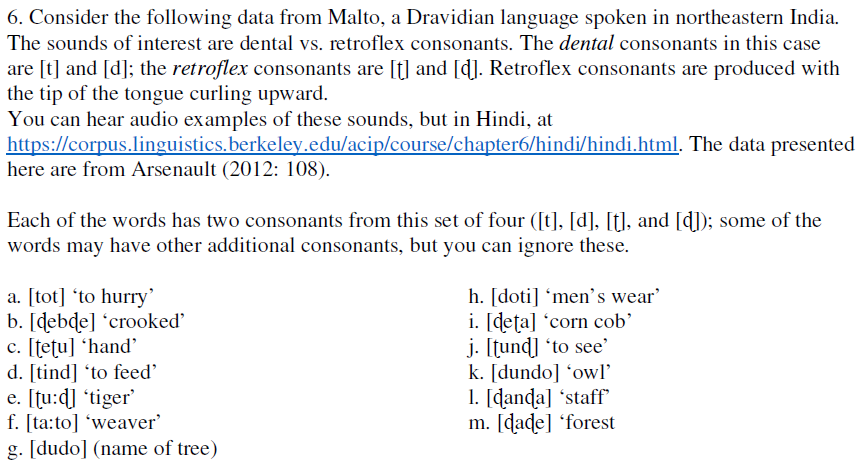
\includegraphics{../images/malto.png}
\end{figure}

\newpage

\begin{center}
\textbf{{\color{red}{\HUGE END OF EXAM}}}\\

\end{center}
\newpage

\begin{center}
\textbf{{\color{blue}{\HUGE START OF EXAM\\}}}

\textbf{{\color{blue}{\HUGE Student ID: 17357\\}}}

\textbf{{\color{blue}{\HUGE 9:10\\}}}

\end{center}
\newpage

{\large Question 1}\\

Topic: Articulatory Phonetics\\
Source: Homework 1, Question 3(a)\\

Could this image be the result of producing the sound represented by the given IPA symbol? Why or why not?\\

{[n]}

\begin{figure}[H]
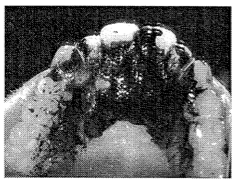
\includegraphics{../images/staticpalatography_stop.png}
\end{figure}

\newpage

{\large Question 2}\\

Topic: Phonological Features\\
Source: Homework 2, Question 1\\

Explain which sound should be removed to make this a natural class (assuming SNAE, except that there are no diphthongs, no [ə] or [ʌ], no syllabic consonants, and no [w̥]), and what the minimum set of features would be to describe the resulting natural class.\\

{[i]}, {[ɪ]}, {[e]}, {[ɛ]}, {[æ]}, {[ɑ]}, {[ɔ]}, {[o]}, {[ʊ]}, {[u]}, {[ʒ]}, {[k]}, {[ɡ]}, {[ŋ]}, {[w]}


\newpage

\begin{center}
\textbf{{\color{red}{\HUGE END OF EXAM}}}\\

\end{center}
\newpage

\begin{center}
\textbf{{\color{blue}{\HUGE START OF EXAM\\}}}

\textbf{{\color{blue}{\HUGE Student ID: 45517\\}}}

\textbf{{\color{blue}{\HUGE 9:20\\}}}

\end{center}
\newpage

{\large Question 1}\\

Topic: Transcription\\
Source: Week 2 Handout, Part II\\

Is this a reasonable transcription of this word? Explain why.\\

<paid>: {[peid]}


\newpage

{\large Question 2}\\

Topic: Skewed Distributions\\
Source: Quiz 4, Question 1\\

L$_X$ (Language X) has three vowels, [i], [a], and [u]. It has bi-syllabic roots like Kikuyu. It does not allow non-identical high vowels to co-occur. Of the following nine logically possible vocalic sequences, which ones should be unattested in L$_X$? Explain why.\\

\begin{itemize} \item {[i...i]} \item {[i...a]} \item {[i...u]} \item {[a...i]} \item {[a...a]} \item {[a...u]} \item {[u...i]} \item {[u...a]} \item {[u...u]} \end{itemize}


\newpage

\begin{center}
\textbf{{\color{red}{\HUGE END OF EXAM}}}\\

\end{center}
\newpage

\begin{center}
\textbf{{\color{blue}{\HUGE START OF EXAM\\}}}

\textbf{{\color{blue}{\HUGE Student ID: 37843\\}}}

\textbf{{\color{blue}{\HUGE 9:30\\}}}

\end{center}
\newpage

{\large Question 1}\\

Topic: Articulatory Phonetics\\
Source: Week 3 Handout, Question 3\\

Explain why the additional vowel below either does or does not belong in the phonetic natural class defined by the original set of SNAE vowels.\\

Original set: {[ɛ]}, {[ɪ]}, {[ʊ]}, {[ɔ]}

Addition: {[ɑ]}


\newpage

{\large Question 2}\\

Topic: Other (pre-midterm)\\
Source: Week 4 Handout, Part II, Question 2(iv)\\

Explain how you would figure out the Swahili word for this English gloss. (To be clear: you do NOT need to give me the Swahili form itself -- just explain the process of figuring it out.)\\

‘She will beat us.’

\begin{figure}[H]
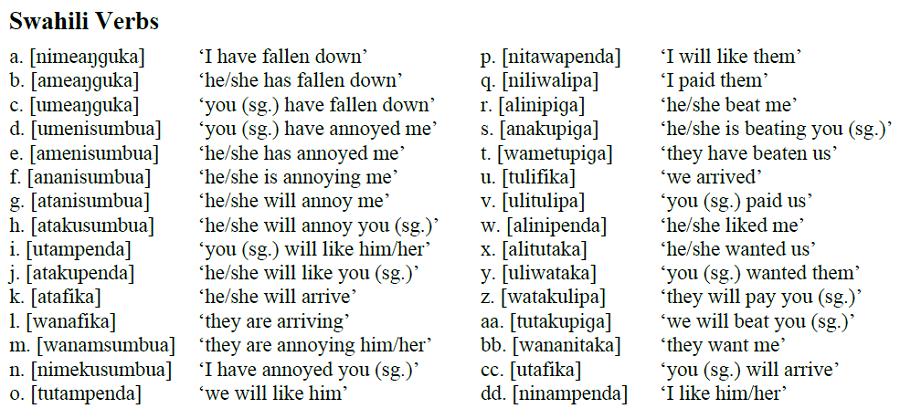
\includegraphics{../images/swahiliverbs.png}
\end{figure}

\newpage

\begin{center}
\textbf{{\color{red}{\HUGE END OF EXAM}}}\\

\end{center}
\newpage

\begin{center}
\textbf{{\color{blue}{\HUGE START OF EXAM\\}}}

\textbf{{\color{blue}{\HUGE Student ID: 17359\\}}}

\textbf{{\color{blue}{\HUGE 9:40\\}}}

\end{center}
\newpage

{\large Question 1}\\

Topic: Articulatory Phonetics\\
Source: Week 3 Handout, Question 3\\

Explain why the additional vowel below either does or does not belong in the phonetic natural class defined by the original set of SNAE vowels.\\

Original set: {[æ]}, {[ɑ]}

Addition: {[ɑɪ]}


\newpage

{\large Question 2}\\

Topic: Transcription\\
Source: Week 2 Handout, Part II, Question 11\\

How would this word be transcribed?\\ (Kathleen will then ask a follow-up question about your transcription.)\\

<square>


\newpage

\begin{center}
\textbf{{\color{red}{\HUGE END OF EXAM}}}\\

\end{center}
\newpage

\begin{center}
\textbf{{\color{blue}{\HUGE START OF EXAM\\}}}

\textbf{{\color{blue}{\HUGE Student ID: 38755\\}}}

\textbf{{\color{blue}{\HUGE 9:50\\}}}

\end{center}
\newpage

{\large Question 1}\\

Topic: Other (pre-midterm)\\
Source: Week 4 Handout, Part II, Question 2(iii)\\

Explain how you would figure out the meaning of this Swahili word. (To be clear: you do NOT need to give me the meaning itself -- just explain the process of figuring it out.)\\

{[tunampenda]}

\begin{figure}[H]
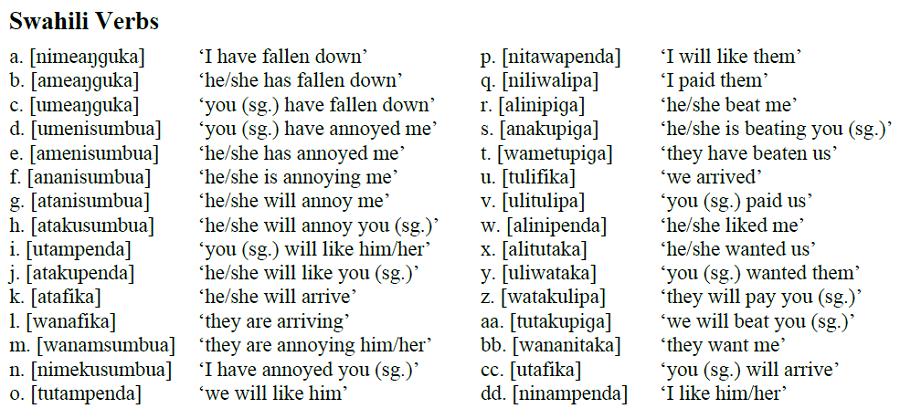
\includegraphics{../images/swahiliverbs.png}
\end{figure}

\newpage

{\large Question 2}\\

Topic: Articulatory Phonetics\\
Source: Homework 1, Question 3(a)\\

Could this image be the result of producing the sound represented by the given IPA symbol? Why or why not?\\

{[t͡ʃ]}

\begin{figure}[H]
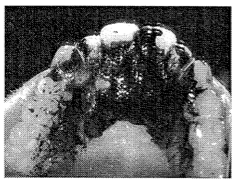
\includegraphics{../images/staticpalatography_stop.png}
\end{figure}

\newpage

\begin{center}
\textbf{{\color{red}{\HUGE END OF EXAM}}}\\

\end{center}
\newpage

\end{document}

